%% 第二章--chapter2.tex
\chapter{代码说明}\label{chap:CodeIntro}
本章将简单说明编译文档所需代码,推荐将本文档与源代码结合起来阅读。

\section{宏包载入选项}\label{sec:loadsty}
主文件\textsf{main.tex}以
\begin{lstlisting}
\usepackage[%
	TextBlack,
	LessTOC,
]{buctthesis}
\end{lstlisting}
命令载入宏包,用以控制全文格式。这里预设了两个选项,可根据需要使用:

\texttt{TextBlack}会将文章超链接和代码块的颜色全部设置为黑色,适合论文最终提交与付梓;
而\texttt{LessTOC}将会把“第一章”之前的部分,即诚信声明、中英文摘要和前言从目录中移除,
这与学校《规定》所展示的样例相同。

\section{前置部分}\label{sec:frontmatter}
\subsection{摘要和关键词}\label{subsec:abstract}
摘要部分的源文件位于\textsf{chapter/abstract.tex},
使用\texttt{abstract}和\texttt{abstracten}环境,在相应位置输入文本即可。

本文档的中、英文摘要分成了两页,
因为若将300字的中文摘要、1500字符的英文摘要及其关键字排版在一页中,行间距会比较狭窄。
若您仍需要排版在同一页,请改用\texttt{abstract*和abstracten*}环境。或将源文件该部分代码
取消注释,同时,为防止摘要部分溢出一页,模板预设了较低的标题间距,但是在内容上的间距未做调整。
若有需要,您可使用 \cmd{setlength\{\cmd{baselineskip}\}\{\}} 命令及参数控制行距。

插入中英文关键词分别使用 \cmd{keywords\{\}}和 \cmd{keywordsen\{\}}命令,
参数即为相应的关键词。但是《规范》中未定义关键词之间的分隔符,
所以模板暂未做任何设置。


\subsection{目录}\label{subsec:content}
在\textsf{buctthesis.tex}中以

\begin{lstlisting}[firstnumber=42]
\tableofcontents
	\end{lstlisting}
命令生成目录。默认编入以下部分:诚信声明、中英文摘要、前言、章、结论、符号说明、
参考文献、附录、节、小节和设计图纸,
不编入以下部分:封面、目录、小小节(subsubsection)及各列表环境、方程、表格和非设计图。

设计图纸需要编号,模板将其编入主目录。命令详情请参见第~\ref{subsec:fig}~小节。


\subsection{前言}\label{subsec:foreword}
前言部分的源代码位于\textsf{chapter/foreword.tex},
使用\texttt{foreword}环境,在相应位置输入文本即可。注意不能在此环境中使用
\cmd{section}等章节命令,结论、翻译、致谢部分同理。
若需要将前言设置为第1页,请将\textsf{buctthesis.tex}文件中
\begin{lstlisting}[firstnumber=45]
%% 前言--foreword.tex
\begin{foreword}
    \addcontentsline{toc}{chapter}{前言}    % 编入目录
    这里是前言。
    点明毕业论文的论题、学术意义以及其与所阅读文献的关系,简要说明文献收集的目的、重点、时空范围、文献种类、核心刊物等方面的内容。

    关于这一部分的设置请参见第 \ref{sec:foreword} 节。
\end{foreword}


	\end{lstlisting}
移至正文部分。

\section{正文}
正文部分各个章节的源文件存放于 \textsf{chapter/} 文件夹,
在 \textsf{buctthesis.tex} 正文部分以

\begin{lstlisting}[numbers=none]
\include{chapter/@*\textsl{filename}@*}
	\end{lstlisting}
命令插入各章节。以此命令插入的文件可以不带扩展名
,此时默认扩展名为 \textsf{.tex}。

使用 \cmd{include} 命令会在读入文件前另起一页。
若不希望这样,可以使用
\begin{lstlisting}[numbers=none]
\input{chapter/@*\textit{filename}@*}
	\end{lstlisting}
此命令相当于纯粹插入文件里的内容。

当随着写作章节增多,每次编译时间也会越来越长。
此时可以选择性地注释已完成的章节,从而快速编译查错。

另外,在格式控制方面,模板已经对各级标题的前后间距做了相应设置。
在章、节标题,用空出相应垂直间距来代替《规范》中的“标准行”。
这一格式控制对全文档都会起作用。
\subsection{字体命令}
\begin{enumerate}
	\item 宋体:北京化工大学 BUCT 1958 或 \textrm{北京化工大学 BUCT 1958}
	\item 粗宋体:{\songti\bfseries 北京化工大学 BUCT 1958} 或 \textbf{\songti 北京化工大学 BUCT 1958}
	\item 黑体:{\bfseries 北京化工大学 BUCT 1958} 或 \textbf{北京化工大学 BUCT 1958}
	\item 粗黑体:{\heiti\bfseries 北京化工大学 BUCT 1958} 或 \textbf{\heiti 北京化工大学 BUCT 1958}
	\item 楷体:{\itshape 北京化工大学 BUCT 1958} 或 \textit{北京化工大学 BUCT 1958}
	\item 仿宋: {\ttfamily 北京化工大学 BUCT 1958} 或 \texttt{北京化工大学 BUCT 1958}
	%\item 微软雅黑与Arial: {\sffamily 北京化工大学 BUCT 1958} 或 \textsf{北京化工大学 BUCT 1958} ,粗体: \textbf{\sffamily 北京化工大学 BUCT 1958} % \footnote{这是为了替代黑体来排版无衬线西文,尽可能不要用其来排版中文。}
\end{enumerate}
\subsection{图片}\label{subsec:fig}
一般的图片插入使用\texttt{figure}环境。
北化的校徽和校名见图~\ref{fig:WholeLogo}。

(机械设计等)设计图纸需要编入目录,使用\cmd{designfig\{\}}命令,
参数为在目录中显示的名称;在目录中的编号与正文编号相同。
在正文中,模板对普通图片和设计图纸的标签和编号没有进行分的设置,即都显示为
如“图 2-1”的形式,但设计图纸在编目时改为如“设计图纸 2-1”的形式。

\begin{figure}[H]
	\centering
	\includegraphics[width=0.4\textwidth]{figure/WholeLogo.ai}
	\caption{校徽和校名}
	\label{fig:WholeLogo}
	\designfig{北化校徽校名}   % 设计图纸加入;且须位于引入图片之后
\end{figure}

一般来说图片使用 \cmd{centering}命令居中对齐。如果需要并排图片,可以使用
\texttt{sub\-figure}环境,使用方法类似。校名见图~\ref{subfig:znname},
校徽见图~\ref{subfig:logo},校名和校徽见图~\ref{fig:wholelogo}。
\begin{figure}[H]
	\centering%
	\begin{subfigure}[b]{6cm}
		
\includegraphics[width=5cm]{figure/ZNName.png}
		\caption{这是校名。如果这个标题比较长,那么它能自动换行。}\label{subfig:znname}
	\end{subfigure}
	\hspace{1cm}
	\begin{subfigure}[b]{2.5cm}
		
\includegraphics[scale=0.4]{figure/Logo.pdf}
		\caption{这是校徽。}\label{subfig:logo}
	\end{subfigure}
	\caption{校名和校徽}\label{fig:wholelogo}
\end{figure}
另外,这里使用了三种不同的图片格式和三种不同的方法来控制所插入图片的大小。

以上命令适合大部分图片的插入。
但不可否认的是,\LaTeX{}对于图文混排的能力是较弱的,如果希望深入了解,推荐~
\href{https://github.com/WenboSheng/epslatex-cn}{\LaTeXe 插图指南}
(中译本第三版)作为参考资料。


\subsection{表格}\label{subsec:tab}
在表 \ref{tab:mainfile} 展示了一个基础的三线表,注意各条横线的粗细是不同的。
使用 \cmd{hline}命令也能划线,但其线宽固定。关于表格内对齐的命令见表~\ref{tab:ATable}。
\begin{table}[H]
	\centering
	\caption{表格的标题}\label{tab:ATable}
	\begin{tabular}{lcr}
		\hline
		左对齐 & 居中对齐 & 右对齐 \\
		\hline
		A      & B        & C      \\
		\hline
	\end{tabular}
\end{table}

另外,三线表生成横线的命令 \cmd{toprule}、\cmd{midrule}和
\cmd{bottomrule}后可以加一个可选参数来实现对线宽的控制。
如果不加参数则为默认值。
此外,两个表格也能横向并列排版,如表~\ref{tab:2tab}。

\begin{table}[H]
	\centering
	\caption{这是一个表格线宽和并列排版的示例}
	\label{tab:2tab}
	\begin{tabular}{ccc}
		\toprule[1.5pt]
		C1    & C2    & C3    \\\midrule[1pt]
		(1,1) & (1,2) & (1,3) \\
		(2,1) & (2,2) & (2,3) \\\midrule[1pt]
	\end{tabular}
	\hspace{1cm}
	\begin{tabular}{ccc}
		\midrule
		C1    & C2    & C3                         \\\toprule
		(1,1) & (1,2) & \multirow{2}{*}{(1,2,3,4)} \\
		(2,1) & (2,2) &                            \\\bottomrule
	\end{tabular}
\end{table}

若要生成稍复杂的表格,本模板已经提供相应的宏包。

如果希望单元格内自动换行以适应列宽,
可以使用\texttt{tabularx}环境,表 \ref{tab:tabularx} 是一个示例。
\begin{table}[htbp]
	\centering
	\begin{minipage}{0.9\textwidth}
		\caption{表格控制列宽及自动折行。有些时候标题会比较长,那么我们可以把表格放到一个小页环境里,从而达到比较好的折行效果。}
		\label{tab:tabularx}
		% 整张表格最大宽度设为文本宽度(由于处于小页,则为0.8倍论文文本宽度);
		% 控制第一、二列列宽,第三列允许折行
		\begin{tabularx}{\textwidth}{p{4em}p{7.5em}X}
			\toprule
									& \multicolumn{1}{l}{原文}         & \multicolumn{1}{l}{翻译}                                                                                         \\
			\cmidrule(l){2-3}
									& 亦余心之所善兮,虽九死其犹未悔。 & For the ideal that I hold dear to my heart,I will not regret a thousand times to die.                           \\
			\cmidrule(l){2-3}
			\multirow{3}{*}{古文翻译} & 不畏浮云遮望眼,自缘身在最高层。 & We have no fear of the clouds that may block our sights as we are already at the top of the height.              \\
			\cmidrule(l){2-3}
									& 苟利国家生死以,岂因祸福避趋之。 & I shall dedicate myself to the interests of the country in life and death irrespective of personal weal and woe. \\
			\bottomrule
		\end{tabularx}
	\end{minipage}
\end{table}

若要在表格中使用脚注,请参见第~\ref{subsec:footnote}小节。

一些在线网站如
~\href{http://www.tablesgenerator.com}{LaTeX Tables Generator}~
可以帮助制作更复杂的表格。


\subsection{公式与数学类环境}\label{subsec:eqandmath}
公式分为编号和不编号的两类。可以使用\texttt{equation}环境为公式编号,如下所示:
\begin{equation}\label{eq:gougu}
	x_{1,2}=\frac{{-b \pm \sqrt{{b^2}-4ac}}}{{2a}}.
\end{equation}
加上 \cmd{label},就能使用 \cmd{ref}或 \cmd{eqref}引用了。
代入\ref{eq:gougu},可解得 \eqref{eq:gougu}。

下面这个是不编号的公式,使用\texttt{equation*}环境:
\begin{equation*}
	\int_{-\infty}^{+\infty}\frac{1}{\sqrt{2\uppi}\sigma}
	\mathrm{e}^{-\tfrac{(x-\mu)^2}{2\sigma^2}} \,\mathrm{d}x =1
\end{equation*}

行内公式可套以美元符号\texttt{\$ \$},如$f(x)=ax^2+bx+c$.
对于上述\texttt{equation*}环境中的公式(即行间公式),可套以双美元符号
\texttt{\$\$ \quad{}\$\$}或\texttt{$\backslash$[ \quad{}$\backslash$]}。
但是并不建议使用前者,因其在\LaTeX{}中并没有完整的重定义,有可能会在某些命令上失效。

关于公式的命令可以参考\textsf{amsmath}宏包说明文档~
\href{https://mirrors.tuna.tsinghua.edu.cn/CTAN/macros/latex/required/amsmath/amsldoc.pdf}
{User's Guide for the amsmath Package}~和~
\href{http://media.cism.it/attachments/ch8.pdf}{Higher Mathematics}。以下举几个例子:

由$\cos 2x=\cos^2x-\sin^2x$ ,		% 函数
则$\boldsymbol{x}=a\bm{i}+b\bm{j}.$	% 粗体,但两种命令效果相似
又因$x\in \mathbb{R} $,			% 字母样式
于是
\[
	\int_a^b f(t)\,\mathrm{d}t = \iint\limits_S g(x,y)\,\mathrm{d}x\mathrm{d}y
	= \iiint\nolimits_D\, \mathrm{d}h.	% 积分号及角标
\]
得
$$\lim_{n \to \infty}\sum_{i=1}^n{\frac{1}{n}}\sin\frac{k}{n}.$$	% 极限、无穷、求和
故
\begin{equation}\label{eq:quadratic}
	\angle A = 90^\circ.			% 角
\end{equation}

若要公式多行对齐,可以使用\texttt{align}环境。下面的例子在等号处对齐:
\begin{align}
	x^2 + y^2 & = 1            \\
	x         & = \sqrt{1-y^2} \\\text{and also }
	y         & =\sqrt{1-x^2}
\end{align}
这会对每一行的公式进行编号。若在\texttt{equation}环境中嵌套\texttt{aligned}环境,加上参数[b]
可以达到多行对齐但只对最后一个式子编号的效果:
\begin{equation}
	\begin{aligned}[b]
		(a + b)^3   & = (a + b) (a + b)^2         \\
					& = (a + b)(a^2 + 2ab + b^2)  \\
					& = a^3 + 3a^2b + 3ab^2 + b^3
	\end{aligned}
\end{equation}

配合使用 \cmd{left.} 与 \cmd{right}\cmd{\}},可以达到使用(右)大括号对方程组编号的效果:
\begin{equation}\left.
	\begin{aligned}
		\nabla  \cdot \mathbf{E} & = \frac{\rho }{\varepsilon _0}                                             \\
		\nabla \times \mathbf{E} & = -\frac{\partial}{\partial t}\mathbf{B}                                   \\
		\nabla  \cdot \mathbf{B} & = 0                                                                        \\
		\nabla \times \mathbf{B} & = \mu_0\mathbf{J}+\mu_0\varepsilon _0\frac{\partial}{\partial t}\mathbf{E}
	\end{aligned} \right\}\text{Maxwell's}
\end{equation}
同理,使用 \cmd{left}\cmd{\}} 与 \cmd{right.},产生的大括号将在左方。

若要对一个方程组内各方程编号,可以使用\texttt{subequations}环境:
\begin{subequations}
	\begin{align}
		\nabla  \cdot \mathbf{E} & = \frac{\rho }{\varepsilon _0}                                             \\
		\nabla \times \mathbf{E} & = -\frac{\partial}{\partial t}\mathbf{B}                                   \\
		\nabla  \cdot \mathbf{B} & = 0                                                                        \\
		\nabla \times \mathbf{B} & = \mu_0\mathbf{J}+\mu_0\varepsilon _0\frac{\partial}{\partial t}\mathbf{E}
	\end{align}
\end{subequations}


再来说说算法。模板载入了\textsf{algorithm}和\textsf{algorithmic}宏包,
并相应地设置了中文。算法~\ref{alg1}~源自\textsf{algorithms}的示例文档。
值得注意的是,算法也是一类“浮动体”,与第~\ref{subsec:code}~小节所使用的
\texttt{lstlisting}环境不同,不容易实现跨页显示。

\begin{algorithm}[htb]
	\setlength{\baselineskip}{1.5em}
	\caption{Calculate $y = x^n$}
	\label{alg1}
	\begin{algorithmic}[1]	  % [1]标注行号
		\REQUIRE $n \geqslant  0 \vee x \neq 0$
		\ENSURE $y = x^n$
		\STATE $y \leftarrow 1$
		\IF{$n < 0$}
		\STATE $X \leftarrow 1 / x$
		\STATE $N \leftarrow -n$
		\ELSE
		\STATE $X \leftarrow x$
		\STATE $N \leftarrow n$
		\ENDIF
		\WHILE{$N \neq 0$}
		\IF{$N$ is even}
		\STATE $X \leftarrow X \times X$
		\STATE $N \leftarrow N / 2$
		\ELSE[$N$ is odd]
		\STATE $y \leftarrow y \times X$
		\STATE $N \leftarrow N - 1$
		\ENDIF
		\ENDWHILE
	\end{algorithmic}
\end{algorithm}



最后,稍微介绍一下数学类的环境。模板加载了\textsf{amsthm}宏包,
且预定义了部分与数学相关的环境,格式及编号如下:
\begin{axiom}
	这是一条axiom,使用\texttt{axiom}环境。
\end{axiom}
\begin{theorem}[某某定理]   % []内为可选参数
	这是一条theorem,使用\texttt{theorem}环境。
\end{theorem}
\begin{corollary}[一条推论]\label{cor:cor1}
	这是一条corollary,使用\texttt{corollary}环境。
\end{corollary}
\begin{proof}
	这是一条proof,使用\texttt{proof}环境。
	\[
		A=\begin{bmatrix}
			a_{11} & \dots  & a_{1n} \\
			\vdots & \ddots & \vdots \\
			0      & \ldots & a_{nn}
		\end{bmatrix}_{n\times n}
	\]

	在证明的最后一行会加上证毕符号,若其位置不合理则需加上命令 \cmd{qedhere}。
	综上所述,推论 \ref{cor:cor1} 成立。
\end{proof}
\begin{remark}
	这是一条remark,使用\texttt{remark}环境
\end{remark}
\begin{assumption}
	这是一条assumption,使用\texttt{assumption}环境。
\end{assumption}
\begin{definition}
	这是一条definition,使用\texttt{definition}环境。
\end{definition}
\begin{property}
	这是一条property,使用\texttt{property}环境。
\end{property}
\begin{proposition}
	这是一条proposition,使用\texttt{proposition}环境。
\end{proposition}
\begin{lemma}
	这是一条lemma,使用\texttt{lemma}环境。
\end{lemma}

以上是模板已经定义了的数学类环境。若需要新定义一个,使用
\begin{lstlisting}[numbers=none]
\newtheorem{@*\emph{environment}@*}{名称}[chapter]
		\end{lstlisting}
如:
\newtheorem{tale}{传说}[chapter]	% 章节编号
\begin{tale}[山经]	  % []内为可选参数
	精卫衔微木,将以填沧海。
\end{tale}
\begin{tale}[海经]
	刑天舞干戚,猛志固常在。
\end{tale}



\subsection{代码}\label{subsec:code}
若要在文中插入代码,简单的代码可以使用原文照列命令~\verb+\verb+或~\verb*@\verb*@,
比如~\verb-i++-、\verb*|int main|,二者区别在于,带*号的将展示代码中的空格。
如果插入代码块,可使用环境\texttt{lstlisting},且可以有如下选择:
\subsubsection{直接在\LaTeX{}中书写代码:}
\begin{lstlisting}[language=C++,caption=Hello World!,label=code:HelloWorld]
/* Hello World C++ */
#include<iostream>
using namespace std;
/*****   main function	*****/
int main()
{
	cout<<"Hello World!"<<endl;		// @*输出 Hello World! ,这里是\LaTeX{}!@*
	return 0;
}
\end{lstlisting}
\subsubsection{引用代码文件,其存放于\textsf{code/}文件夹里:}
\lstinputlisting[
	language=C++,
	caption=你好,世界!,
	label=code:HelloWorld2
]{code/helloworld.cpp}

本模板以 Times New Roman 字体书写代码,关键字以粗体标出,
而注释使用斜体。

另外,代码中的``逃逸字符''设置为\texttt{@*},可以返回至\LaTeX{}中,
如代码 \ref{code:HelloWorld}。


\subsection{化学类}
模板加载了\textsf{mhchem}宏包,方便了化学(方程)式的书写。
使用命令 \cmd{ce\{\}}把化学(方程)式括起来。
\subsubsection{简单化学式}
\begin{table}[H]
	\centering
	\begin{tabular}{llllll}
		\ce{H2O}    & \ce{Sb2O3}  & \ce{KCr(SO4)2.12H2O} & \ce{CrO4^2-}                & \ce{[AgCl2]-}              & \ce{^{0}_{-1}M^{-}} \\
		\ce{$n$H2O} & \ce{H2(aq)} & \ce{KCr(SO4)2*12H2O} & \ce{Fe(CN)_{$\frac{6}{2}$}} & \ce{$cis${-}[PtCl2(NH3)2]} & \ce{\alpha-Al2O3}   \\
	\end{tabular}
\end{table}
\subsubsection{含键化学式}
\begin{table}[H]
	\centering
	\begin{tabular}{llll}
		\ce{A-B=C#D}                           & \ce{A\bond{-}B\bond{=}C\bond{#}D} & \ce{A\bond{1}B\bond{2}C\bond{3}D} & \ce{A\bond{~}B\bond{~-}C} \\
		\ce{A\bond{~--}B\bond{~=}C\bond{-~-}D} & \ce{A\bond{...}B\bond{....}C}     & \ce{A\bond{->}B\bond{<-}C}        &                           \\
	\end{tabular}
\end{table}
\subsubsection{化学方程式}
\begin{table}[H]
	\centering
	\begin{tabular}{llll}
		\ce{A ->[H2O] B} & \ce{A <=>[{上方文字}][{text below}] B} & \ce{A ->[$x$][$x_i$] B} & \ce{A v B (v) -> C ^ D (^)} \\
	\end{tabular}
\end{table}
\subsubsection{其他}
\begin{itemize}
	\item 标注(可能对 CJK 文字不支持):
			\ce{Zn^2+
			<=>[+ 2OH-][+ 2H+]
			$\underset{\text{amphoteres Hydroxid}}{\ce{Zn(OH)2 v}}$
			<=>[+ 2OH-][+ 2H+]
			$\underset{\text{Hydroxozikat}}{\ce{[Zn(OH)4]^2-}}$
			}
	\item 对于化学方程式等的编号,与数学方程相似:
			$$\ce{2H2O ->[{electrify}] 2H2 ^ + O2 ^}$$
			\begin{equation}
					K^\ominus  = \ce{\frac{[Hg^2+][Hg]}{[Hg2^2+]}}
			\end{equation}
\end{itemize}

对于至于有机化学结构式等,尽管有一些宏包可以绘制,但使用图片插入可能是一个更好
的选择。

\section{文献引用和参考文献}\label{sec:bib}
\subsection{在文章中引用文献}
模板使用 \cmd{cite\{\}}命令实现上标、方括号以“顺序编码制”引用参考文献,
这是学校《规范》的要求。一个例子。\cite{abbott2016observation}而使用
\cmd{inlinecite\{\}}命令则不使用上标引用,\cmd{nocite}
命令则指明不引用但需要列出的参考文献。

同一处引用多个文献时,应将各篇文献的引用标签一同写在 \cmd{cite} 命令中,
并以西文逗号“,”分隔各标签。所产生的样式为:当在同一处引用两篇参考文献时,
引用序号将以西文逗号分隔;
当多余两篇且连续时,将标示起止序号并以短划线相连。这\cite{texbook,latexrumen}
又是\cite{texbook,latexrumen,gbt7714-2005}一个例子。\cite{abbott2016observation,texbook,latexrumen,buctthesis}


\subsection{论文的参考文献章节}
本模板已在\textsf{buctthesis.tex}中使用
\begin{lstlisting}[firstnumber=52]
\bibliographystyle{gbt7714-2005}
\bibliography{thesisbib.bib}
	\end{lstlisting}
来增加符合格式要求的参考文献章节。
为罗列各条参考文献,您需要在\textsf{thesisbib.bib}文件中增删需引用的文献数据。

注意:至少需要引用一篇参考文献,否则执行完全编译可能会引起编译错误。如果暂不需要参考文献,
请将主文件里的这两行删除或注释掉。

关于如何编辑\textsf{thesisbib.bib},
可以使用\href{http://scholar.google.com.cn/}{谷歌学术}\footnote{亦可以访问国内镜像站}
或\href{http://xueshu.baidu.com}{百度学术}两种方式(方法类似)导入\BibTeX{}:
\begin{itemize}
	\item 在搜索框中搜索论文题目/作者/DOI等,以确定所引用的论文;
	\item 点击\emph{引用},如图~\ref{fig:addbib}:
			\begin{figure}[htbp]
				\centering
				\caption{谷歌学术中的``引用''}
				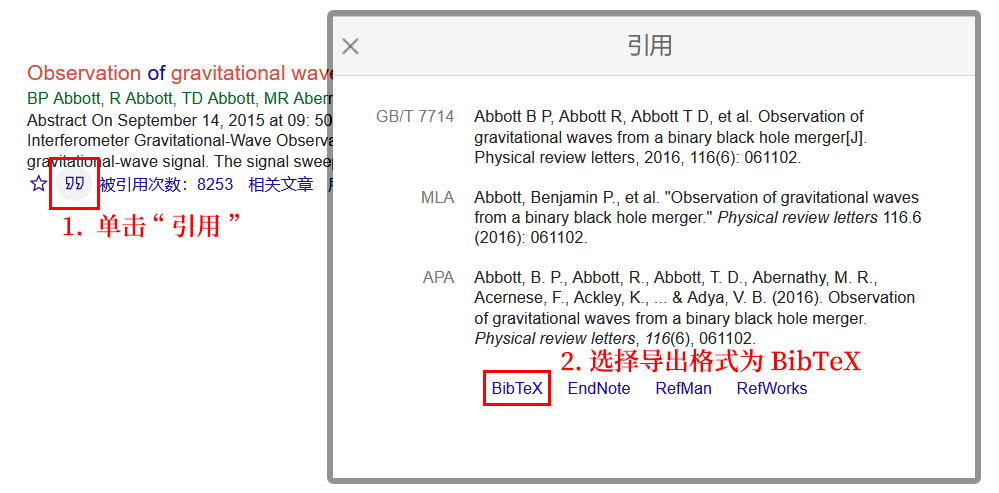
\includegraphics[width=10cm]{figure/AddBib.png}
				\label{fig:addbib}
			\end{figure}
	\item 在弹出框中,单击最下方 Bibtex 的链接;
	\item 在弹出的网页中复制所有代码至\textsf{thesisbib.bib},并根据需要做一些改动;
	\item 在您的论文中使用 \cmd{cite\{\}}引用相应的文献。
\end{itemize}

举个例子:在网页中将
\begin{lstlisting}
@article{abbott2016observation,
	title={Observation of gravitational waves from a binary black hole merger},
	author={Abbott, Benjamin P and Abbott,% ...
	},
	journal={Physical review letters},
	volume={116},
	number={6},
	pages={061102},
	year={2016},
	publisher={APS}
}
	\end{lstlisting}
复制进 \textsf{thesisbib.bib},在您的论文中使用
\cmd{cite\{abbott2016observation\}}即可引用此文献。
这里的 “abbott2016observation”是该篇参考文献的引用标签,可以修改。
再来一个\cite{ashirov2008tetramerization} ,
网络上的资源引用\cite{buctthesis},等。

另外,参考文献格式控制文件\textsf{gbt7714-2005.bst}开源于
\href{https://github.com/Haixing-Hu/GBT7714-2005-BibTeX-Style}{GitHub},
其参考文献的著录可以用于参考。

\section{后置部分}\label{sec:backmatter}
\subsection{附录}\label{sec:app}
在\textsf{buctthesis.tex}中以
\begin{lstlisting}[firstnumber=68]
\appendix
		\end{lstlisting}
命令作为附录部分的开始。与正文类似,只需往\textsf{chapter/app1.tex}等加入内容即可,
除了编号使用大写字母之外都一样。见附录 \ref{app:1}。

\subsection{符号说明}\label{sec:deno}
符号说明部分的源文件位于\textsf{chapter/denotation.tex},使用\texttt{denotation}环境。
《规范》中未详细规定符号说明部分的格式,模板使用了一个可跨页的长表格,
不过无需对表格进行设置或	划线,直接在环境里填入内容即可。环境的两个参数
\textit{SymbWid}和\textit{DenoWid}分别是“符号”和“说明”二列的宽度,用于在必要时调整。

\begin{lstlisting}
\begin{denotation}{@*\textit{SymbWid}@*}{@*\textit{DenoWid}@*}
	符号1   &   说明1   \\
	符号2   &   说明2   \\
\end{denotation}
		\end{lstlisting}
所生成的样式请参考本文的符号说明部分。

\subsection{致谢}
致谢部分的源文件位于\textsf{chapter/acknowledgement.tex},
使用\texttt{acknowledgement}环境,往里面写入感谢的话就可以啦。
\begin{lstlisting}
\begin{acknowledgement}
	% Words here.
	% ...
\end{acknowledgement}
		\end{lstlisting}

\section{其他}\label{sec:other}

\subsection{脚注}\label{subsec:footnote}
本模板采用带圈数字脚注,计数跨章重置,使用命令 \cmd{footnote}。
前方高能\footnote{我是可爱的脚注}。

有些情况下(比如在表格环境、各种盒子内)使用 \cmd{footnote}并不能正确生成脚注。
我们可以分两步进行,先使用 \cmd{footnotemark} 为脚注计数,
再在合适的位置用 \cmd{footnotetext} 生成脚注。比如表~\ref{tab:ftnt1}。
\begin{table}[H]
	\centering
	\caption{脚注示例1}
	\label{tab:ftnt1}
	\begin{tabular}{llll}
		\hline
		人之初                & 性本善 & 性相近 & 习相远 \\
		苟 \footnotemark 不教 & 性乃迁 & 教之道 & 贵以专 \\
		\hline
	\end{tabular}
\end{table}
\footnotetext{苟:如果}

还有一种手动在表格底生成脚注的方法,见表~\ref{tab:ftnt2}。
\begin{table}[htbp]
	\centering
	\caption{脚注示例2}
	\label{tab:ftnt2}
	\begin{minipage}[H]{7.5cm}
		\begin{tabular}{llll}
			\hline
			昔孟母 & 择邻处 $^{*}$       & 子不学 & 断机杼 \\
			窦燕山 & 有义方 $^{\dagger}$ & 教五子 & 名俱扬 \\
			\hline
		\end{tabular}\\[3pt]
		\footnotesize
		$^*$脚注1\\
		$^\dagger$脚注2
	\end{minipage}
\end{table}

\subsection{列表环境}\label{subsec:items}
本模板提供了三种列表环境:不编号的\texttt{itemize}、编号的\texttt{enumerate}
和使用关键字的\texttt{description}环境。在文档的中英文摘要部分分别展示了
基础的编号和不编号的列表环境;上面三种列表环境可以嵌套使用(至多四层),
且会自动处理不同层次的缩进和编号,如下所示:
\begin{itemize}
	\item 一条
	\item 次条
	\item 这一条可以分为\dots
			\begin{itemize}
				\item 子一条
			\end{itemize}
\end{itemize}
稍复杂一点的,如:
\begin{enumerate}
	\item 中文
		\begin{description}
			\item[文言文] 古代汉语
			\item[白话文] 现代汉语
				\begin{enumerate}
					\item 口语
						\begin{enumerate}
							\item 普通话
							\item 方言
						\end{enumerate}
					\item 书面语
				\end{enumerate}
		\end{description}
	\item English
\end{enumerate}

注意:一级编号列表环境最多罗列10条,否则标签会显示错误。%,否则到第11条时,标签将从第10条的\ding{201}到第11条的\ding{202}
